% *******************************************************************************
% générer la biblio: chmod +x check-biblio.pl
% générer le pdf: make
% suppression des fichiers temporaires: make clean
% suppression de tous les fichiers temporaires: make cleanall 
% *******************************************************************************

\documentclass[a4paper]{article}
\usepackage[utf8]{inputenc}
\fontencoding{T1}
\usepackage[pdftex]{graphicx, color}
\usepackage[english,frenchb]{babel}
\usepackage{url, pdfpages}
\graphicspath{ {fig/pdf/} }

%-------------------------------------------------------------------------------
% Page de garde
%-------------------------------------------------------------------------------

\newlength{\larg}
\setlength{\larg}{14.5cm}

\begin{document}

\includepdf[pages=-]{cov}
\newpage
\tableofcontents
\newpage

%-------------------------------------------------------------------------------
% Shell environment
%-------------------------------------------------------------------------------
%\newenvironment{shell}
%{\rule{1ex}{1ex}\hspace{\stretch{1}}}
%{\hspace{\stretch{1}}\rule{1ex}{1ex}}


%*******************************************************************************
\section*{Introduction}
%*******************************************************************************

Ce projet a comme objectif la réalisation de recueils de chansons
proposant paroles et accords de guitare pour facilement jouer ses
morceaux préférés au coin du feu.

L'objectif est simple: obtenir un rendu homogène et agréable de toutes
ses tablatures. Si vous faîtes souvent des soirées musicales, je suis
certain que vous avez déjà dû pester contre toutes ces feuilles
volantes, les partitions mal imprimées, les fautes de frappe, un
accord qui sonnerait mieux en le jouant d'une autre façon, etc \dots
En tous cas, moi oui. Cela fait donc quelques années que j'essaye de
faire des carnets de chant. Après avoir fait quelques essais mitigés
avec les outils bureautiques classiques et propriétaires (Word© et
Publisher© pour ne citer qu'eux), \LaTeX m'a enfin permis de faire à
peu près ce que je voulais.

%*******************************************************************************
\section{Procédure d'installation sous Linux}
%*******************************************************************************

%------------------------------------------------------------------------------
\subsection{Dépendances}
%------------------------------------------------------------------------------

Ce recueil de chansons a été écrit en \LaTeX. Pour compiler vous-même
vos propres chansons, vous devez disposer de make, perl, python,
pdflatex et d'un viewer pdf. Si vous êtes sous Debian/Ubuntu:

\paragraph{Dépendances obligatoires}
\begin{verbatim}
//LaTeX
$ sudo apt-get install texlive-base texlive-lang-french texlive-latex-extra
//Indexes en python
$ sudo apt-get install python
\end{verbatim}

\paragraph{Dépendances recommandées}
\begin{verbatim}
//Pour la génération des partitions Lilypond
$ sudo apt-get install lilypond
//Pour récupérer les sources du projet via Git
$ sudo apt-get install git-core
\end{verbatim}

%------------------------------------------------------------------------------
\subsection{Récupération des sources}
%------------------------------------------------------------------------------

Il y a deux façons de récupérer les fichiers source du carnet de
chants:
\begin{itemize}
\item télécharger l'archive tar.gz
\item utiliser le gestionnaire de version Git
\end{itemize}

\paragraph{Depuis l'archive tar.gz}
Il faut extraire le contenu de l'archive dans le répertoire de votre
choix. De manière générale, évitez les chemins contenant des espaces
ou des caractères spéciaux. Dans ce manuel, le répertoire de travail
est supposé être: \$HOME/songbook pouvant être noté
/home/user/songbook ou \~/songbook .
\begin{verbatim}
$ cd $HOME
$ wget http://www.patacrep.com/files/songbook.tar.gz
$ tar xzvf songbook.tar.gz
\end{verbatim}

\paragraph{Depuis le dépôt Git}
Il est conseillé d'utiliser la méthode utilisant le gestionnaire de
version Git pour des raisons pratiques.
\begin{verbatim}
$ cd $HOME
$ git clone git://git.lohrun.net/songbook.git
\end{verbatim}

%------------------------------------------------------------------------------
\subsection{Compilation}
%------------------------------------------------------------------------------

Un \emph{makefile} automatise tout le processus de compilation. La
génération du songbook ne demande donc qu'un: 

\begin{verbatim}
$ cd $HOME/songbook
$ make all
\end{verbatim}

Quelques options de base du makefile:

\paragraph{\$ make clean} 
supprime tous les fichiers de logs et les fichiers générés à part les
books finaux (pdf).

\paragraph{\$ make cleanall}
supprime tous les fichiers générés y compris les pdf.

\paragraph{\$ make lilypond}
génère dans ./lilypond les pdf de chaque partition lilypond (.ly)
trouvée dans ./lilypond. Il est nécessaire d'avoir installé
\emph{lilypond} au préalable.

\paragraph{\$ make book.pdf}
la compilation de tous les carnets pouvant être longue, si seule une
version précise vous intéresse, vous pouvez lancer la compilation d'un
seul fichier pdf. Notez que la commande ``make'' sans option correspond à un ``make chordbook.pdf''. À la place de \emph{book.pdf}, vous pouvez mettre:
\begin{itemize}
\item chordbook.pdf
\item lyricbook.pdf
\item lilypondbook.pdf
\item volume-1-cb.pdf
\item volume-1-lb.pdf
\item volume-1-ll.pdf
\item volume-2-cb.pdf
\item volume-2-lb.pdf
\item volume-2-ll.pdf
\item naheulbeuk-cb.pdf
\item naheulbeuk-lb.pdf
\item naheulbeuk-ll.pdf
\end{itemize}

%------------------------------------------------------------------------------
\subsection{Mise à jour}
%------------------------------------------------------------------------------

Pour maintenir à jour la version du songbook, vous pouvez télécharger
la dernière version en mise en ligne de l'archive tar.gz ou, si vous
avez utilisé Git pour récupérer les sources:
\begin{verbatim}
$ cd $HOME/songbook
$ git pull
\end{verbatim} 

%*******************************************************************************
\section{Songbook client}
%*******************************************************************************

%------------------------------------------------------------------------------
\subsection{Présentation et interface}
%------------------------------------------------------------------------------

Une interface graphique, réalisée en Qt4/C++, est disponible pour
faciliter la création d'un recueil de chansons personnalisé.

\begin{figure}
  \centering
  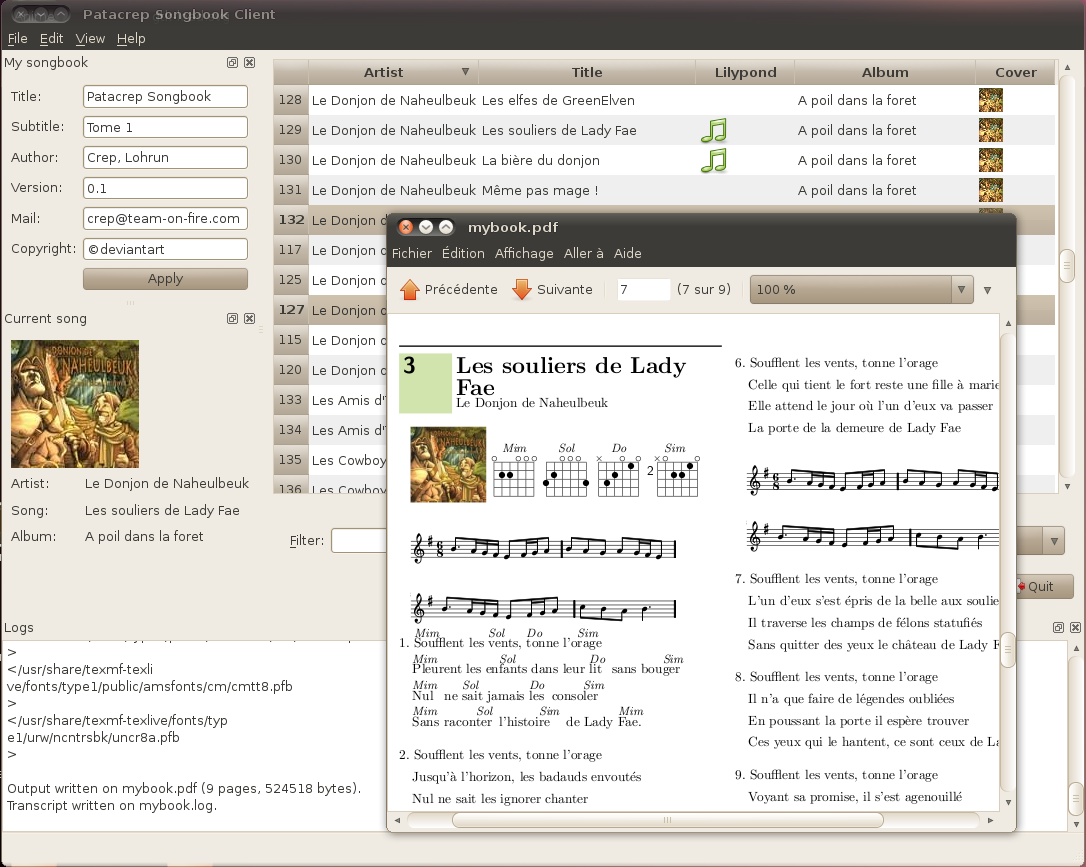
\includegraphics[width=\textwidth]{songbook-client2}
  \caption{Qt4 client pour la génération des songbooks.}
  \label{fig:sb-client}
\end{figure}

Une présentation du projet peut se trouver sur:
\begin{itemize}
\item \url{http://www.ohloh.net/p/songbook-client}
\item \url{http://github.com/crep4ever/songbook-client}
\end{itemize}

%------------------------------------------------------------------------------
\subsection{Installation depuis les sources}
%------------------------------------------------------------------------------

\paragraph{Dépendances}
\begin{verbatim}
sudo apt-get install build-essential cmake qt4-qmake qt4-dev-tools libqt4-sql-sqlite
\end{verbatim}

\paragraph{Installation}
\begin{verbatim}
$ cd $HOME
$ git clone git://github.com/crep4ever/songbook-client.git
$ cd songbook-client
$ make
$ sudo make install
\end{verbatim}

%------------------------------------------------------------------------------
\subsection{Installation depuis le paquet Debian}
%------------------------------------------------------------------------------

Un paquet Debian (.deb) est disponible pour faciliter le processus
d'installation du songbook-client. 

\begin{verbatim}
$ cd $HOME
$ wget http://www.patacrep.com/files/songbook-client-01_amd64.deb
$ sudo dpkg -i songbook-client-01_amd64.deb
\end{verbatim}

Note: si le lien n'est pas à jour ou si vous êtes sur une autre
architecture, allez dans le répertoire
\url{http://www.patacrep.com/files/} et récupérez le fichier
.deb adéquat.

%------------------------------------------------------------------------------
\subsection{Configuration}
%------------------------------------------------------------------------------

Pour lancer l'application, faîtes Alt+F2 songbook-client ou dans un
terminal:
\begin{verbatim}
$ songbook-client
\end{verbatim}

Une fois l'application lancée, il est important:
\begin{itemize}
\item d'indiquer le chemin du songbook dans les préférences (par
  exemple /home/user/songbook). Ce répertoire devant impérativement
  contenir le makefile et le répertoire songs/ contenant les chansons
  disponibles;
\item de resynchroniser la base de données avec le nouveau répertoire
  indiqué (Fichier/Synchroniser).
\end{itemize}

%------------------------------------------------------------------------------
\subsection{Problèmes divers}
%------------------------------------------------------------------------------

N'hésitez pas à faire remonter les bugs que vous pouvez rencontrer sur
le forum ou par mail directement. 

\paragraph{Sqlite} Si vous voyez une boîte de dialogue
d'avertissement se lancer au démarrage de l'application indiquant que
le support de sqlite est nécessaire, vous ne pourrez pas utiliser
l'interface. Vérifiez que votre système dispose bien du support Qt de sqlite.

\paragraph{Pas de partitions}
Si la compilation de votre recueil de chansons n'intègre pas les
partitions malgré l'option \emph{Lilypond} correctement cochée dans les
préférences, vérifiez que Lilypond est bien installé sur votre système. 

\paragraph{Liste des chansons vide} Vérifiez que le chemin d'accès au
patacrep songbook est correctement renseigné dans Édition/Préférences.
Le chemin indiqué doit contenir impérativement le makefile et le
répertoire songs/


%*******************************************************************************
\section{Comment écrire une chanson}
%*******************************************************************************

%------------------------------------------------------------------------------
\subsection{À propos de \LaTeX}
%------------------------------------------------------------------------------

\LaTeX est un logiciel de traitement de texte qui produit un document
bien formaté d'après des sources (un simple fichier texte). Cela
permet à l'utilisateur de se concentrer sur le contenu plutôt que sur
la forme. C'est un langage de programmation basé sur un système de
commandes et/ou de balises.

Une commande commence part un antislash ``$\backslash$'' suivi du nom
de la commande. Ensuite viennent les arguments, si il y en a, entre
accolades (obligatoires) ou crochets (optionnels).

%------------------------------------------------------------------------------
\subsection{Éléments principaux}
%------------------------------------------------------------------------------

Une chanson est un simple fichier texte ``'ma\_chanson.sg'' que l'on
place dans le répertoire songs/Artiste. Les espaces n'étant
pas tolérés, veillez à utiliser des underscores \_. L'entête d'un fichier
.sg se présente de la manière suivante:

\begin{verbatim}
\beginsong{Titre}[by=Artiste,cov=album-cover]
\end{verbatim}

Les arguments \emph{Titre}, \emph{Artiste} et \emph{album-cover} sont
à renseigner pour chaque nouvelle chanson. \emph{album-cover} désigne
un fichier \emph{album-cover.jpg} devant se trouver dans le même
répertoire que le fichier .sg.  La chanson se compose d'une succession
de couplets (verse en anglais) et de refrains (chorus). Un couplet est
donc encadré par les balises \emph{beginverse} et \emph{endverse}. De
la même manière, un refrain se trouve entre les balises
\emph{beginchorus} et \emph{endchorus}.  Les paroles sont écrites
normalement entre le $\backslash$begin et le $\backslash$end. Pour
préciser sur quelle syllabe un accord doit être joué, on utilise une
commande spéciale. Par exemple, la commande $\backslash$[Mi] produira
un Mi au dessus de la syllabe suivante. Vous pouvez utiliser n'importe
quel texte pour désigner un accord.

\begin{center}
\begin{verbatim}
\beginverse
His \[Rém]steely skin is covered
By \[Fa]centuries of dust
\[Do]Once he was a great one
\[Rém]Now he's dull and rust
\endverse
\end{verbatim}
\end{center}

Chaque chanson se termine avec la commande \emph{endsong}.

\begin{verbatim}
\endsong
\end{verbatim}

%------------------------------------------------------------------------------
\subsection{Notation des accords}\label{sect:about}
%------------------------------------------------------------------------------

Par défaut, l'accord est majeur (Do fait référence à l'accord de Do
majeur). Les accords mineurs sont précisés par un ``m'' minuscule.  Le
symbole bémol ($\flat$) est représenté en utilisant le caractère ``\&''.  Le
dièse ($\sharp$) est codé par le caractère ``\#''. Les autres notations sont
simplement ajoutées comme des caractères à l'accord principal. Par
exemple, l'accord de ``La bémol mineur'' est noté ``La\&m''.


%------------------------------------------------------------------------------
\subsection{Exemple complet}
%------------------------------------------------------------------------------

Voici un exemple complet pouvant être utilisé comme point de départ
pour écrire une nouvelle chanson.

\begin{verbatim}
\songcolumns{2}
\beginsong{Sad robot}[by=Pornophonique,cov=8-bit-lagerfeuer]

\cover
\gtab{Rém}{X00231}
\gtab{Fa}{1:022100}
\gtab{Do}{X32010}

\beginverse
His \[Rém]steely skin is covered
By \[Fa]centuries of dust
\[Do]Once he was a great one
\[Rém]Now he's dull and rust
\endverse

\beginverse*
An oily tear he's crying
Can you feel the pain
Of the sad, sad robot
And it's driving him insane
\endverse

\beginchorus
Sad, sad robot \rep{3}
All alone
\endchorus

\beginchorus
He's a sad, sad robot \rep{3}
He's so alone
\endchorus

\endsong
\end{verbatim}

%*******************************************************************************
\section{Mise en page avancée}
%*******************************************************************************

%------------------------------------------------------------------------------
\subsection{Agencement en colonnes}
%------------------------------------------------------------------------------

La commande \emph{songcolumns} détermine le nombre de colonnes sur
lequel sera présenté la chanson. Elle s'utilise juste avant la
commande \emph{beginsong}. Vous pouvez indiquer le nombre de colonnes
à utiliser pour écrire votre chanson (généralement 1, 2 ou 3). Par
convention, utilisez 2 colonnes par défaut.

\begin{verbatim}
\songcolumns{2}
\beginsong{Titre}[by=Artiste,cov=album-cover]
\end{verbatim}

%------------------------------------------------------------------------------
\subsection{Caractères spéciaux}
%------------------------------------------------------------------------------

Quelques caractères doivent être codés différemment en utilisant des
commandes \LaTeX pour un meilleur résultat. Les deux exemples
principaux sont les 3 points (...) et le caractère \oe{}. Pour
représenter ces caractères, vous devez utiliser respectivement les
commandes ${\backslash dots}$ et ${\backslash oe}$ (ou utiliser le
caractère utf8 ``œ''). On utilise des accolades autour des commandes de
sorte que les commandes puissent être insérées où vous le désirez sans
interférer avec le reste du texte. Voir aussi
section\,\ref{sect:utilitaires}.

%------------------------------------------------------------------------------
\subsection{Ch\oe{}urs et répétitions}
%------------------------------------------------------------------------------

Pour produire un signe de répétition vous pouvez utiliser la commande
$\backslash$rep. Pour faire répéter quatre fois une ligne utilisez la
commande suivante à la fin de la ligne. La commande $\backslash$echo
fait référence à des ch\oe{}urs (ou similaire).

\begin{verbatim}
Hallelujah \echo{Hallelujah} \rep{4}
\end{verbatim}

%------------------------------------------------------------------------------
\subsection{Numérotation des couplets}
%------------------------------------------------------------------------------

La numérotation se fait automatiquement pour chaque \emph{beginverse}
rencontré. Cependant, il est parfois plus lisible de scinder un
couplet en deux parties, la deuxième partie ne devant pas être
numérotée. Pour cela on utilise la commande \emph{beginverse*}.
 
\begin{verbatim}
\beginverse
His \[Rém]steely skin is covered
By \[Fa]centuries of dust
\[Do]Once he was a great one
\[Rém]Now he's dull and rust
\endverse

\beginverse*
An oily tear he's crying
Can you feel the pain
Of the sad, sad robot
And it's driving him insane
\endverse
\end{verbatim}

%------------------------------------------------------------------------------
\subsection{Représentation des accords}
%------------------------------------------------------------------------------

Étant donné qu'un accord de guitare peut se jouer de plusieurs façons
différentes et qu'il est parfois judicieux de privilégier telle ou
telle position, le songbook permet de représenter schématiquement ces
accords en début de chanson. On utilise la commande \emph{gtab} juste
avant le premier couplet ou refrain. Voici quelques exemples classiques:

\begin{verbatim}
\gtab{Ré}{XX0232}
\gtab{Mi}{022100}
\gtab{Do}{3:002220}
\end{verbatim}

\begin{itemize}
\item les 6 chiffres correspondent aux 6 cordes de la
guitare (Mi, La, Ré Sol, Si, Mi);
\item la valeur du chiffre indique la fret (case) sur laquelle on
  appuie;
\item 0 désigne une corde jouée à vide;
\item X indique que la corde ne doit pas être jouée;
\item une valeur avant un ``:'' désigne un barré: \emph{3:} indique
un barré de trois frets.
\end{itemize}


%*******************************************************************************
\section{Partager votre travail}
%*******************************************************************************

Si vous ajoutez une chanson au carnet de chant, pourquoi ne pas nous
envoyer votre fichier. Nous y jetterons un \oe{}il et serons enchantés
de l'ajouter au carnet de chant ``officiel''. Comme toujours les
contributeurs sont les bienvenus.

\begin{itemize}
\item envoyez directement vos remarques par mail à
  \url{crep@team-on-fire.com};
\item utilisez le forum comme bon vous semble;
\item envoyez des patch;
\end{itemize}

%-------------------------------------------------------------------------------
\subsection{Création d'un patch}
%-------------------------------------------------------------------------------

Le meilleur moyen est de nous envoyer un patch. Techniquement, un
patch est un simple fichier texte qui indique les opérations
(ajout/suppression) qui ont été opérées sur un fichier texte. Un
exemple tout simple a l'aspect suivant:

\begin{verbatim}
index 3fcce15..b4edcc1 100644
--- a/songs/Cat_Stevens/The_wind.sg
+++ b/songs/Cat_Stevens/The_wind.sg
@@ -7,7 +7,7 @@

-\[Do] I listen to the \[Fa]wind,
+\[Ré] I listen to the \[Sol]wind,
\end{verbatim}

Vous voyez rapidement qu'après les premières lignes qui servent à
identifier le fichier sur lequel on a travaillé, j'ai remplacé:
\begin{verbatim}
-\[Do] I listen to the \[Fa]wind,
\end{verbatim}
par
\begin{verbatim}
+\[Ré] I listen to the \[Sol]wind,
\end{verbatim}

Concrètement, si vous avez suivi la procédure d'installation,
vous devriez avoir un répertoire \$HOME/songbook/ contenant toutes les
sources du carnet de chant. Maintenant, vous avez repéré une erreur
dans la chanson songs/artiste/chanson.sg. Ouvrez le fichier
correspondant avec votre éditeur de texte préféré, faîtes votre
correction, enregistrez, fermez. Puis, dans un terminal:

\begin{verbatim}
$ cd $HOME/songbook
$ git diff -u songs/artiste/chanson.sg > patch
\end{verbatim}

Cela va vous créer un nouveau fichier "patch" qui contiendra
l'ensemble des modifications que vous avez apportées à votre
chanson. Plus qu'à nous l'envoyer !

%-------------------------------------------------------------------------------
\subsection{Création de votre version du songbook}
%-------------------------------------------------------------------------------

Si vous prévoyez de faire beaucoup de modifications ou de rejoindre
activement le développement du songbook, le système de patch n'est pas
forcément adapté et il vaut mieux dans ce cas partir sur votre propre
version du songbook. La meilleure solution consiste à faire un
\emph{fork} du projet Git et de l'héberger sur le web si vous comptez
le partager. Des solutions web gratuites permettent d'héberger de tels
projets. Par exemple:
\begin{itemize}
\item \url{http://github.com}
\item \url{http://gitorious.org}
\end{itemize}

Il suffit alors de nous communiquer l'adresse de votre dépôt Git de
façon à ce que nous puissions récupérer vos changements.



%%*******************************************************************************
%\section{Accords usuels}
%%*******************************************************************************
%
%%------------------------------------------------------------------------------
%\subsection{Accords majeurs}
%%------------------------------------------------------------------------------
%
%
%%------------------------------------------------------------------------------
%\subsection{Accords mineurs}
%%------------------------------------------------------------------------------
%
%
%%------------------------------------------------------------------------------
%\subsection{Accords de 7ème}
%%------------------------------------------------------------------------------


%*******************************************************************************
\section{Intégration des partitions avec Lilypond}
%*******************************************************************************

%------------------------------------------------------------------------------
\subsection{Lilypond}
%------------------------------------------------------------------------------

La documentation du projet Lilypond est très
claire et se trouve sur le site \url{http://lilypond.org/}.
Voici néanmoins quelques concepts de base:

\begin{itemize}
\item les lettres a, b, c, d, e, f, g représente les notes la, si, do,
  ré, mi, fa, sol;
\item un chiffre derrière une lettre en indique la durée (2=blanche, 4=noire,
  8=croche) et un point après un chiffre désigne une note pointée;
\item \emph{ais}, \emph{bes} désignent un \emph{la dièse} et un \emph{si bémol}
\item \emph{'} et \emph{,} servent à monter/descendre d'une octave;
\end{itemize}

Lilypond est généralement empaqueté pour les distributions
GNU/Linux. Pour des distributions basées Debian/Ubuntu, l'installation
se fait par:

\begin{verbatim}
$ sudo apt-get install lilypond
\end{verbatim}


%------------------------------------------------------------------------------
\subsection{Intégration au songbook}
%------------------------------------------------------------------------------

Si vous voulez rajouter une ligne mélodique dans une chanson, vous
pouvez utiliser lilypond pour générer la partition. Créez pour cela un
nouveau fichier ma\_partition.ly dans le répertoire songbook/lilypond.
Il faut inclure le fichier d'en-tête ``header'' et définir l'option
paper-height de façon à ce que la partition produite tienne sur une
page avec le moins de blanc possible. Une première estimation est de
compter 1.6cm pour une ligne. Puis, écrivez votre partition entre
accolades comme dans l'exemple suivant (Tom Sawyer) pour obtenir le
résultat en Fig.~\ref{fig:lilypond}:

\begin{verbatim}
\include "header"
\paper{paper-height = 3.3\cm}
{
  \key c \major
  \time 2/4
  \relative c''{
    e4 c g'2 a4 a8. a16 g8 e4 c8 a'4 a8. a16 g8 f e c d2~ d4
    e8 f g4 g8. g16 f8 e d c a c4 a8 g4 c8 d e8 g4 g,8 e' e d d c2
  }
}
\end{verbatim}

\begin{figure}
  \centering
  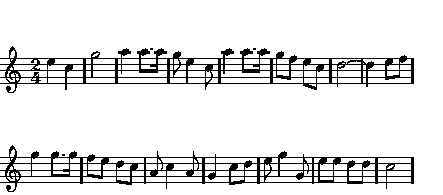
\includegraphics[width=0.8\textwidth]{lilypond}
  \caption{Intégration de partitions avec Lilypond.}
  \label{fig:lilypond}
\end{figure}

Enfin, pour insérer votre partition dans une chanson, insérez la ligne
suivante à l'endroit désiré dans ma\_chanson.sg:

\begin{verbatim}
\lilypond{ma_partition}
\end{verbatim}

Toutes les partitions lilypond présentes dans le répertoire
songbook/lilypond sont automatiquement générées par le makefile. Pour
construire le songbook incluant les partitions lilypond, il suffit de
faire:

\begin{verbatim}
$ make lilypond
$ make lilypondbook.pdf 
\end{verbatim}


%*******************************************************************************
\section{Utilitaires}\label{sect:utilitaires}
%*******************************************************************************

Des scripts utilitaires sont disponibles dans le répertoire
songbook/utils. On les exécute classiquement en faisant:

\begin{verbatim}
$ cd $HOME/songbook
$ ./utils/script.sh
\end{verbatim}

\paragraph{Resize cover}
Permet de redimensionner automatiquement tous les fichiers .jpg du
répertoire songbook/songs correspondant aux pochettes des albums. À
exécuter après l'ajout d'une nouvelle pochette (jpg recommandé, png
supporté).

\paragraph{Latex preprocessing}
Applique un ensemble de règles automatiques pour les notations \LaTeX
de certains caractères et pour les notations d'accords.
À exécuter après l'ajout d'une nouvelle chanson pour être sûr de
respecter les standards du songbook.

\paragraph{New songs list}
Permet de récupérer la liste des chansons ajoutées depuis la dernière
version.

\paragraph{Volume\,2}
Permet de générer la liste des chansons qui ne sont pas dans le volume\,1.

\paragraph{Make html}
Génère la liste de toutes les chansons au format html.


%*******************************************************************************
\section{Conseils aux débutants}
%*******************************************************************************

%------------------------------------------------------------------------------
\subsection{Les accords de base}
%------------------------------------------------------------------------------

Les accords de base sont les accords qui se jouent sans barré au
niveau des premières frets:

\begin{itemize}
\item Accords Majeurs:\\ 
  Do (X32010), Sol (320003), La (X02220), Ré (XX0232), Mi (022100)\\
\item Accords Mineurs:\\
  Mim (022000), Lam (X02210), Rém (XX0231)\\
\item Accord Septième:\\
  Mi7 (020100), Sol7 (320001), Ré7 (XX0212), La7 (X02020), Si7 (X21202)\\
\end{itemize}

Donc déjà, il est bon de savoir jouer et enchainer assez rapidement
ces accords là. Le mieux c'est de chercher des morceaux avec ces
accords et de s'entraîner dessus.  À part pour l'accord de ré, les
cordes marquées d'un X peuvent quand même sonner.  C'est juste qu'on
préfère généralement attaquer par la fondamentale de l'accord (ex:
note do pour l'accord de do majeur).  À propos des différentes
notations d'accords, il s'agit juste d'une question de sonorité ou de
pragmatisme. On est toujours libre de jouer l'accord de la façon qui
nous arrange le plus.

%------------------------------------------------------------------------------
\subsection{Transposer un morceau}
%------------------------------------------------------------------------------

L'idée, c'est de toujours pouvoir se ramener à un enchaînement
d'accords que l'on maîtrise.  Pour transposer un morceau, c'est pas
dur il suffit d'appliquer le même décalage à tous les accords.  Par
exemple, pour la chanson du hérisson, si on décale de 2 tons 1/2: Sim,
Sol, Fa$\sharp$7 se transposent en Mim, Do, Si7.  Et miracle, ces
accords là ne demandent plus de barrés !

%------------------------------------------------------------------------------
\subsection{Les barrés}
%------------------------------------------------------------------------------

Bon, le coup de transposer les accords, c'est un bon exercice pour
jongler avec les accords et leurs enchaînements mais de temps en
temps, ça ne suffit pas, il reste toujours des barrés qui apparaissent
et c'est quand même mieux de jouer les vrais accords. Donc attaquons
la fameuse technique du barré. Tout bon débutant qui se respecte
commence par le barré de mi \dots pour faire un fa. Oui, en fait,
barré c'est se servir de son index comme capo pour transposer l'accord
qu'on fait dessous (avec un doigt en moins).

Exemple: l'accord de Fa se joue 133211. Il est cependant noté 1:022100
dans le carnet de chant car c'est un barré de Mi (022100) sur la
première fret.  Donc l'idée, c'est d'appuyer bien fort avec son index
en travers de toutes les cordes et d'utiliser annulaire, ptit doigt,
majeur pour appuyer sur les 3 cordes demandées. À savoir qu'il y a
essentiellement 4 types de barrés.  Dans l'ordre de difficulté: barrés
de Mi (022100), Lam (002210), Mim (022000), La (002220).

%------------------------------------------------------------------------------
\subsection{Les rythmes}
%------------------------------------------------------------------------------

Contrairement à ce que l'on pourrait croire, il est bien plus
difficile de maîtriser la main droite que la main gauche.
Voici quelques motifs assez passe-partout pour vos morceaux.

\paragraph{Rythme ``à la Brassens''} Il s'agit d'alterner une basse (pouce)
avec 3 aiguës simultanées (index, majeur, annulaire), 2 ou 4 fois par
accord. En général, les 3 aiguës sont les 3 cordes aiguës 4,5,6 (Sol,
Si, mi) et la basse alterne entre les cordes 1,2,3 (Mi, La, Ré) mais
souvent dans l'ordre 2,1.

\paragraph{Rythme ``arpège''} Il s'agit d'un motif note-à-note qui
accompagne très bien les chansons calmes. Chaque guitariste a le
sien, voici l'ordre des cordes à jouer pour le mien: 2 654 654 6. En
gros, on fait une basse avec le pouce, puis deux descentes aiguës avec
annulaire, majeur, index et on finit par la plus aiguë.

\paragraph{Rythme ``feu de camp''} Quand il faut gratter, le premier
piège est de suivre le rythme du chant. Gardez un rythme constant !
//arf, j'arrive pas à expliquer ... //


%------------------------------------------------------------------------------
\subsection{Les techniques du fourbe}
%------------------------------------------------------------------------------

Alors je ne sais pas trop si ça peut aider ou non mais j'ai mis au
point mes propres techniques secrètes de débutant faignant. Elles sont
quand même relativement déconseillées dans la mesure ou ce sont de
mauvaises habitudes pas académiques dont on a du mal à se défaire.

\paragraph{L'accord de Sol}
Arf, voilà mon premier échec à la guitare. Après avoir enchainé des
accords de La et de Mi pendant 3 heures je m'essaye au sol. Position
ok, ça sonne bien. Manque de pot, impossible d'enchainer ça
rapidement.  Du coup, remarquant qu'un Sol se jouait en 320003, je me
suis dit qu'avec un seul doigt, j'avais déjà 4 cordes sur 6. Donc j'ai
commencé en jouant mes Sol en XX0003 avec seulement l'annulaire et ça
sonnait très bien. 1 an plus tard, j'ai réalisé qu'en mettant le pouce
sur la première corde ça marchait encore mieux (3X0003) donc voilà la
technique de la pince pour l'accord de Sol qui fait beaucoup rire les
vrais guitaristes quand ils me voient jouer.

\paragraph{L'accord de Fa}
Après avoir contourné le problème du Sol s'est posé celui du Fa. La
c'est pareil, impossible de tenir la position barrée plus de deux
nanosecondes sans hurler de douleur.  Je me suis dit, trouvons une parade:
le semi barré.  En fait, quand on regarde la théorie du barré, c'est
pas bien optimisé puisque l'index appuie sur toutes les cordes donc on
appuie 2 fois sur certaines cordes (index 111111, autres doigts 033200)
Donc en fin de comptes, l'index sert seulement pour les cordes 1,5 et
6. Au diable la première, mon index fera 5 et 6 et ce sera suffisant.
Ça donne des Fa comme ça: X33211 avec l'index qui écrase seulement les
deux dernières cordes. Bon, autant je fais encore mes Sol avec mon
pouce, autant j'ai appris à faire des barrés proprement.


\end{document}
